%\addcontentsline{toc}{chapter}{Appendices}

% The \appendix command resets the chapter counter, and changes the chapter
% numbering scheme to capital letters.
\appendix
\chapter{Plots and generated text}
\label{Appendix:output}

\section{Plots}

\begin{figure}[!htbp]
  \centering
  \begin{subfigure}[b]{0.55\textwidth}
    \centering
    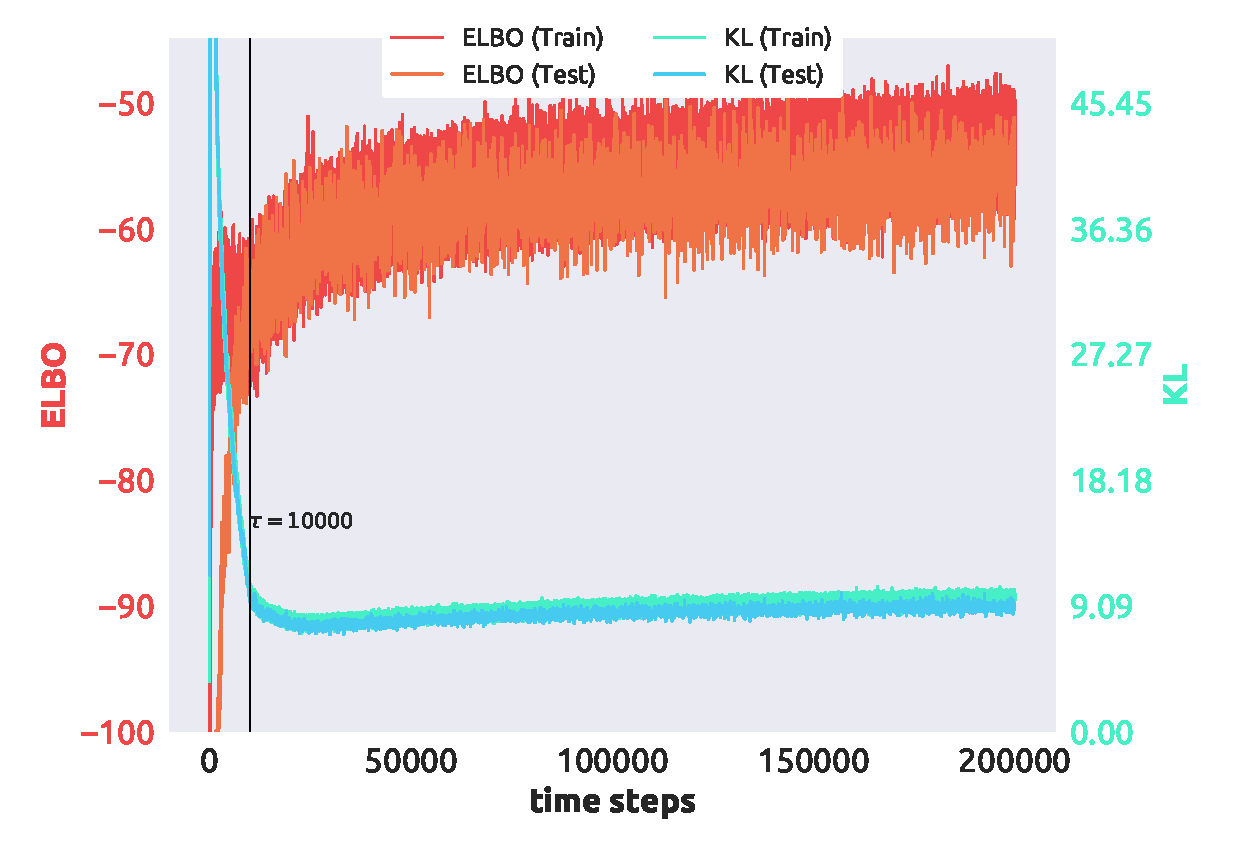
\includegraphics[width=1.0\textwidth]{mlp_reconstruction}
    \caption{Plot for $\mathcal{M}_{M1}$}
    \label{fig:recon_MLP}
  \end{subfigure}
  \begin{subfigure}[b]{0.55\textwidth}
    \centering
    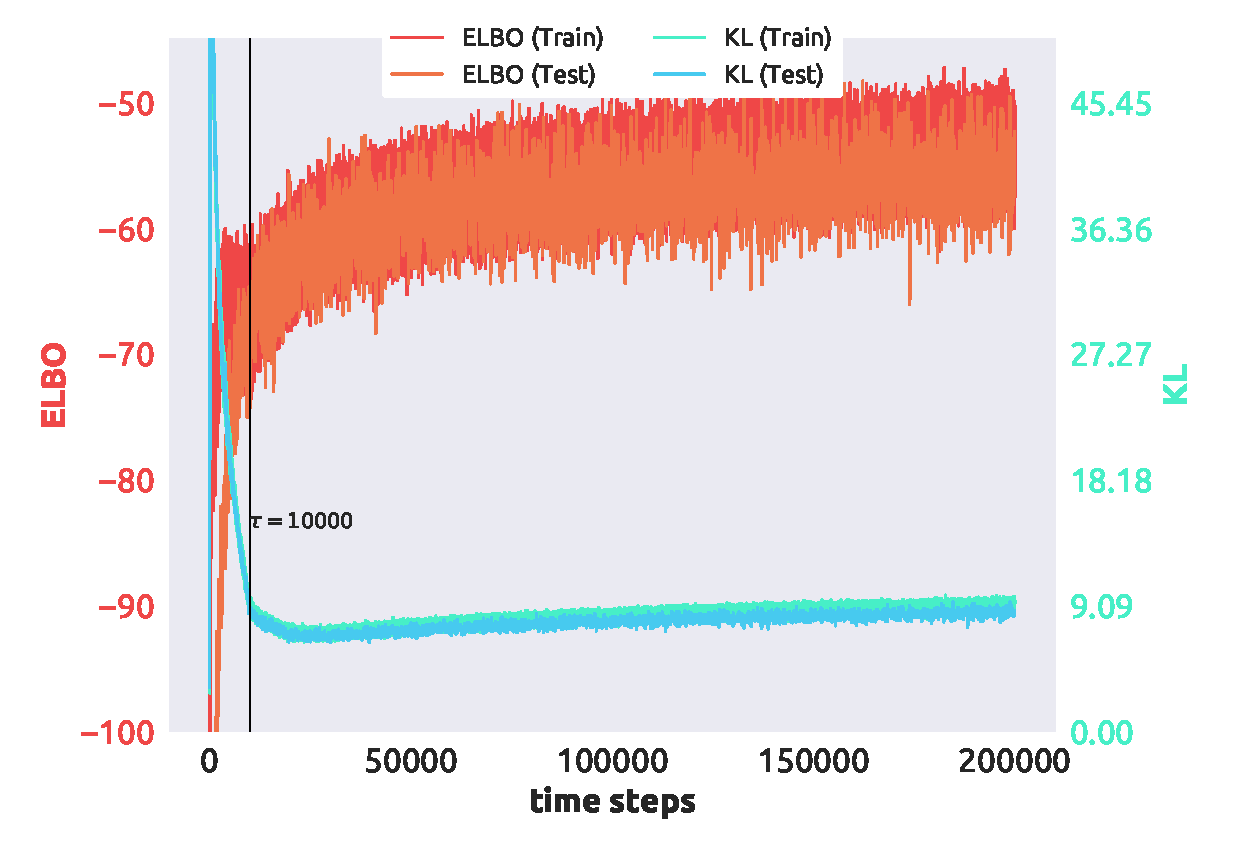
\includegraphics[width=1.0\textwidth]{rnn_reconstruction}
    \caption{Plot for $\mathcal{M}_{M2}$}
    \label{fig:recon_RNN}
  \end{subfigure}
  \begin{subfigure}[b]{0.55\textwidth}
    \centering
    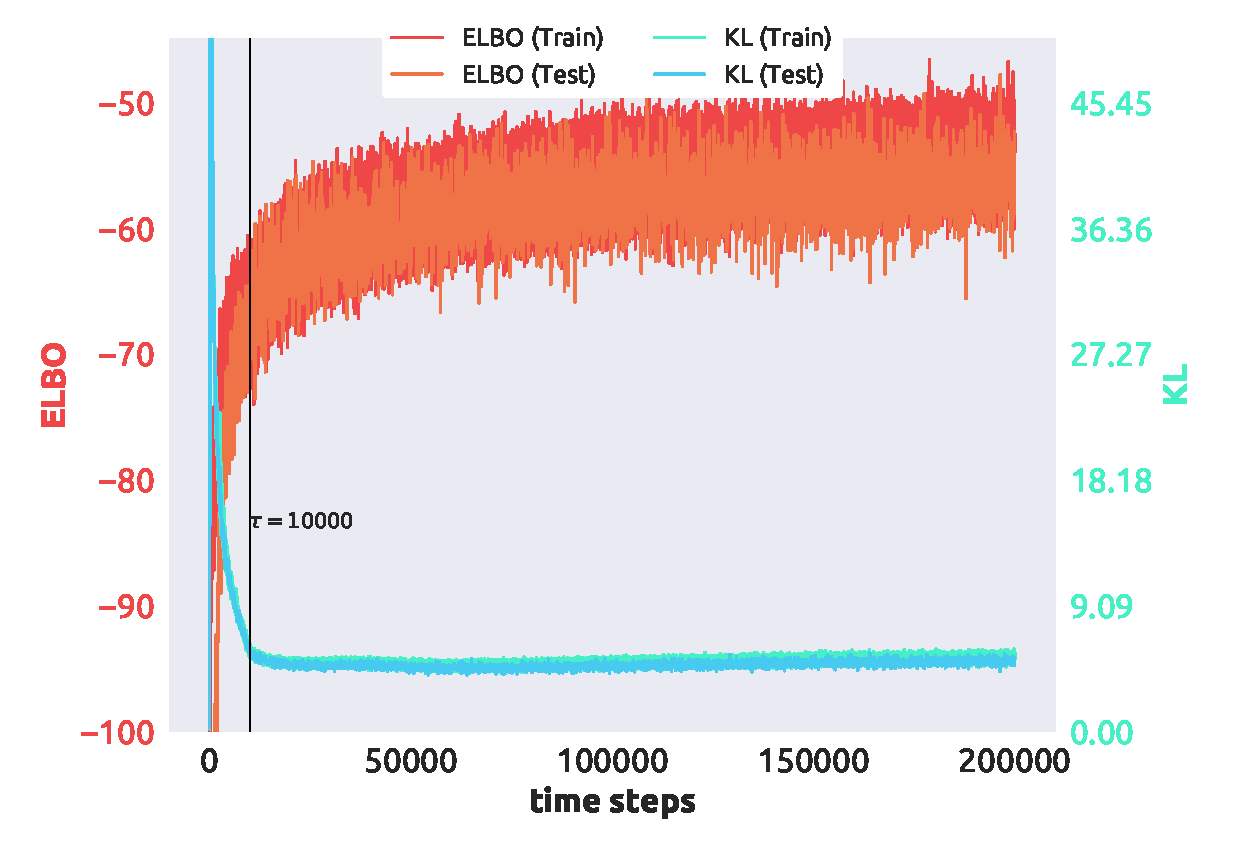
\includegraphics[width=1.0\textwidth]{wavenet_reconstruction}
    \caption{Plot for $\mathcal{M}_{M3}$}
    \label{fig:recon_WaveNet}
  \end{subfigure}
  \caption{Plots of the SGVB estimate of ELBO (Labelled ELBO in plots)
      together with the KL divergence $\KL{q_{\bm{\varphi}}(\bm{z} |
        \bm{x})}{p_{\bm{\theta}}(\bm{z})}$ for the different models for
      Mono-language models. The
      vertical line specifies the end of the KL-annealing.}
\end{figure}

\begin{figure}[!htbp]
  \centering
  \begin{subfigure}[b]{0.5\textwidth}
    \centering
    \includegraphics[width=1.0\textwidth]{full_fig_mlp_wavenet_translation_fr_en_20-08-17_18:16}
    \caption{Plot for $\mathcal{M}_{T1}$}
    \label{fig:translate_M1}
  \end{subfigure}%
  \begin{subfigure}[b]{0.5\textwidth}
    \centering
    \includegraphics[width=1.0\textwidth]{full_fig_mlp_wavenet_translation_fr_en_22-08-17_11_21}
    \caption{Plot for $\mathcal{M}_{T2}$}
    \label{fig:translate_M2}
  \end{subfigure}
  \begin{subfigure}[b]{0.5\textwidth}
    \centering
    \includegraphics[width=1.0\textwidth]{full_fig_mlp_wavenet_translation_fr_en_28-08-17_20_22}
    \caption{Plot for $\mathcal{M}_{T3}$}
    \label{fig:translate_M3}
  \end{subfigure}%
  \begin{subfigure}[b]{0.5\textwidth}
    \centering
    \includegraphics[width=1.0\textwidth]{full_fig_mlp_wavenet_translation_fr_en_big_dataset_29-08-17_10:36}
    \caption{Plot for $\mathcal{M}_{T4}$}
    \label{fig:translate_M4}
  \end{subfigure}
  \caption{Plots of the SGVB estimate of ELBO (Labelled ELBO in plots)
      together with the KL divergence $\KL{q_{\bm{\varphi}}(\bm{z} |
        \bm{x})}{p_{\bm{\theta}}(\bm{z})}$ for the different models for
      Twin-language models. The
      vertical line specifies the end of the KL-annealing.}
\end{figure}

\FloatBarrier

\section{Generated Sentences}

We let (T) stand for the true sentence, and (G) for the generated sentence.

\begin{table}
  \centering
  \begin{tabular}{|L{14cm}|} 
    \hline
    Sampled sentences from prior\\ [0.5ex] 
    \hline\hline
    the vote will take place on the debate , the council , and the commission .\\
    \hline
    i have already received a number of questions .\\
    \hline
    why , we have to be able to get the right to get the right ?\\
    \hline
  \end{tabular}
  \caption{Sampled sentences (EN) using the prior $p(\bm{z})$ of model $\mathcal{M}_{M1}$.}
\end{table}

\begin{table}
  \centering
  \begin{tabular}{|L{14cm}|} 
    \hline
    Sampled sentences from posterior\\ [0.5ex] 
    \hline\hline
    (T) faced with this situation , europe has a decision to make .\\
    (G) in the council , we are faced with a situation .\\
    \hline
    (T) now , that process certainly requires a reliable police force .\\
    (G) this is a new process , the european union is needed .\\
    \hline
    (T) as i am pleased to say that the commission is going to be done .\\
    (G) as i say , i shall be here with the presidency .\\
    \hline
  \end{tabular}
  \caption{Sampled sentences (EN) using the recognition model
    $q_{\bm{\varphi}}(\bm{z} | \bm{x})$ of model $\mathcal{M}_{M1}$.}
\end{table}

\begin{table}
  \centering
  \begin{tabular}{|L{14cm}|} 
    \hline
    Sampled sentences from prior\\ [0.5ex] 
    \hline\hline
    what is the result of the vote , and i am not going to be taken .\\
    \hline
    as you believe that the commission is right , we need to be transparent .\\
    \hline
    i am not a great deal of a great deal of a great deal .\\
    \hline
  \end{tabular}
  \caption{Sampled sentences (EN) using the prior $p(\bm{z})$ of model $\mathcal{M}_{M2}$.}
\end{table}

\begin{table}
  \centering
  \begin{tabular}{|L{14cm}|} 
    \hline
    Sampled sentences from posterior\\ [0.5ex] 
    \hline\hline
    (T) i hope that we will continue to support the commission .\\
    (G) i hope we shall be able to maintain this cooperative approach throughout the subsequent presidencies .\\
    \hline
    (T) i agree with the need to support efficiency and effectiveness in the various education systems .\\
    (G) i believe that we need to improve the need for greater transparency and efficiency .\\
    \hline
    (T) this decline is encouraging news .\\
    (G) the situation is a very important .\\
    \hline
  \end{tabular}
  \caption{Sampled sentences (EN) using the recognition model
    $q_{\bm{\varphi}}(\bm{z} | \bm{x})$ of model $\mathcal{M}_{M2}$.}
\end{table}

\begin{table}
  \centering
  \begin{tabular}{|L{14cm}|} 
    \hline
    Sampled sentences from prior\\ [0.5ex] 
    \hline\hline
    the commission is not the same thing , and the same .\\
    \hline
    ( the sitting was closed at UNK p.m . )\\
    \hline
    the european union 's aim is to be welcomed .\\
    \hline
  \end{tabular}
  \caption{Sampled sentences (EN) using the prior $p(\bm{z})$ of model $\mathcal{M}_{M3}$.}
\end{table}

\begin{table}
  \centering
  \begin{tabular}{|L{14cm}|} 
    \hline
    Sampled sentences from posterior\\ [0.5ex] 
    \hline\hline
    (T) the eu should stop these payments immediately .\\
    (G) we must not be taken into account .\\
    \hline
    (T) that is the inescapable conclusion we must draw .\\
    (G) the commission is very important .\\
    \hline
    (T) mr president , thank you very much for this debate .\\
    (G) i would like to thank you for your attention .\\
    \hline
  \end{tabular}
  \caption{Sampled sentences (EN) using the recognition model
    $q_{\bm{\varphi}}(\bm{z} | \bm{x})$ of model $\mathcal{M}_{M3}$.}
\end{table}

\begin{table}
  \centering
  \begin{tabular}{|L{14cm}|} 
    \hline
    Sampled sentences from prior\\ [0.5ex] 
    \hline\hline
    in my view the european union has been said .\\
    \hline
    now we are all UNK ! \\
    \hline
    as far ' s and UNK to being UNK to UNK UNK , to the UNK UNK .\\
    \hline
  \end{tabular}
  \caption{Sampled sentences (EN) using the prior $p(\bm{z})$ of model $\mathcal{M}_{T1}$.}
\end{table}

\begin{table}
  \centering
  \begin{tabular}{|L{14cm}|} 
    \hline
    Sampled sentences from posterior\\ [0.5ex] 
    \hline\hline
    (T) i find it sad that there are meps who are trying to weaken the commission ' s proposal .\\
    (G) i find it is that the commission , however , the commission is not in the commission .\\
    \hline
    (T) mr president , commissioner , ladies and gentlemen , what is this debate actually about ?\\
    (G) mr president , commissioner , ladies and gentlemen , what is going to do about ?\\
    \hline
    (T) mrs UNK was the rapporteur at the time .\\
    (G) mrs UNK has to be of no to UNK .\\
    \hline
  \end{tabular}
  \caption{Sampled sentences (EN) using the recognition model
    $q_{\bm{\varphi}}(\bm{z} | \bm{x}, \bm{y})$ of model $\mathcal{M}_{T1}$.}
\end{table}

\begin{table}
  \centering
  \begin{tabular}{|L{14cm}|} 
    \hline
    Sampled sentences from prior\\ [0.5ex] 
    \hline\hline
    madame la présidente , ce problème n'est pas tout une intervention des femmes .\\
    \hline
    pouviez , notre groupe aussi pour un communication pour cette approche .\\
    \hline
    lançons , UNK a la parole de la commission .\\
    \hline
  \end{tabular}
  \caption{Sampled sentences (FR) using the prior $p(\bm{z})$ of model $\mathcal{M}_{T1}$.}
\end{table}

\begin{table}
  \centering
  \begin{tabular}{|L{14cm}|} 
    \hline
    Sampled sentences from posterior\\ [0.5ex] 
    \hline\hline
    (T) il est regrettable , selon moi , que certains députés essayent d'affaiblir l'initiative de la commission .\\
    (G) je suis néanmoins qu'il est que la commission que l'on est une proposition pas de la commission .\\
    \hline
    (T) monsieur le président , madame la commissaire , chers collègues , de quoi traite vraiment ce débat ?\\
    (G) monsieur le président , madame la présidente , monsieur le commissaire , dont nous avons ce débat ?\\
    \hline
    (T) à l’époque , c’est mme UNK qui était rapporteur .\\
    (G) à occupé de UNK , cela était de UNK .\\
    \hline
  \end{tabular}
  \caption{Sampled sentences (FR) using the recognition model
    $q_{\bm{\varphi}}(\bm{z} | \bm{x}, \bm{y})$ of model $\mathcal{M}_{T1}$.}
\end{table}

\begin{table}
  \centering
  \begin{tabular}{|L{14cm}|} 
    \hline
    Sampled sentences from prior\\
    \hline\hline
    mr president , i see on this report , in the vote .\\
    \hline
    i would like to thank wreckage to hope to be for the european union to be made .\\
    \hline
    you must be able to make for one of one .\\
    \hline
  \end{tabular}
  \caption{Sampled sentences (EN) using the prior $p(\bm{z})$ of model $\mathcal{M}_{T2}$.}
\end{table}

\begin{table}
  \centering
  \begin{tabular}{|L{14cm}|} 
    \hline
    Sampled sentences from posterior\\ [0.5ex] 
    \hline\hline
    (T) there is a real guerrilla war in progress .\\
    (G) there is a great is the union is .\\
    \hline
    (T) however , later on , while i was asleep , i dreamt of mrs roth-behrendt .\\
    (G) however , as of course , i have , i welcome , i have about .\\
    \hline
    (T) mr president , there is essentially nothing surprising about the situation today .\\
    (G) mr president , there is no longer in the european parliament .\\
    \hline
  \end{tabular}
  \caption{Sampled sentences (EN) using the recognition model
    $q_{\bm{\varphi}}(\bm{z} | \bm{x}, \bm{y})$ of model $\mathcal{M}_{T2}$.}
\end{table}

\begin{table}
  \centering
  \begin{tabular}{|L{14cm}|}
    \hline
    Sampled sentences from prior\\
    \hline\hline
    je tiens à présent à la commission à la commission .\\
    \hline
    nous UNK donc cette décision au conseil .\\
    \hline
    par conséquent ce sont les citoyens .\\
    \hline
  \end{tabular}
  \caption{Sampled sentences (FR) using the prior $p(\bm{z})$ of model $\mathcal{M}_{T2}$.}
\end{table}

\begin{table}
  \centering
  \begin{tabular}{|L{14cm}|} 
    \hline
    Sampled sentences from posterior\\ [0.5ex] 
    \hline\hline
    (T) une guérilla énorme est en cours .\\
    (G) la russie est en effet est .\\
    \hline
    (T) puis , je me suis quand même UNK , et j'ai rêvé de mme roth-behrendt .\\
    (G) et je tigre , je me UNK , je me UNK , et je me UNK .\\
    \hline
    (T) monsieur le président , la situation d'aujourd'hui n'a au fond rien d'étonnant .\\
    (G) monsieur le président , la situation n'est pas la situation sont la situation .\\
    \hline
  \end{tabular}
  \caption{Sampled sentences (FR) using the recognition model
    $q_{\bm{\varphi}}(\bm{z} | \bm{x}, \bm{y})$ of model $\mathcal{M}_{T2}$.}
\end{table}

\begin{table}
  \centering
  \begin{tabular}{|L{14cm}|} 
    \hline
    Sampled sentences from prior\\
    \hline\hline
    to those member states , for proposal for UNK would not support the most people .\\
    \hline
    we would like to make a new measures that of this point .\\
    \hline
    that is something we are now today .\\
    \hline
  \end{tabular}
  \caption{Sampled sentences (EN) using the prior $p(\bm{z})$ of model $\mathcal{M}_{T3}$.}
\end{table}

\begin{table}
  \centering
  \begin{tabular}{|L{14cm}|} 
    \hline
    Sampled sentences from posterior\\ [0.5ex] 
    \hline\hline
    (T) it is a compromise .\\
    (G) this is a compromise .\\
    \hline
    (T) that is why this aid programme needs to be made a top priority .\\
    (G) that is why the only to do is about to be in UNK .\\
    \hline
    (T) yet it is a country that is important to europe .\\
    (G) yet it is an UNK of an UNK for europe .\\
    \hline
  \end{tabular}
  \caption{Sampled sentences (EN) using the recognition model
    $q_{\bm{\varphi}}(\bm{z} | \bm{x}, \bm{y})$ of model $\mathcal{M}_{T3}$.}
\end{table}

\begin{table}
  \centering
  \begin{tabular}{|L{14cm}|} 
    \hline
    Sampled sentences from prior\\
    \hline\hline
    il convient est souvent de nouvelles à cet aspect pas les UNK à cet accord .\\
    \hline
    cependant , nous sommes tous , tout , à bien se fait .\\
    \hline
    c'est pourquoi j'ai également que notre travail à faire dans notre dans ce sens .\\
    \hline
  \end{tabular}
  \caption{Sampled sentences (FR) using the prior $p(\bm{z})$ of model $\mathcal{M}_{T3}$.}
\end{table}

\begin{table}
  \centering
  \begin{tabular}{|L{14cm}|} 
    \hline
    Sampled sentences from posterior\\ [0.5ex] 
    \hline\hline
    (T) c’est un compromis .\\
    (G) c’est un compromis .\\
    \hline
    (T) c'est pourquoi ce programme d'assistance doit avant tout être prioritaire .\\
    (G) c'est pourquoi ce programme doit être une question au niveau .\\
    \hline
    (T) mais c'est un pays important pour l'europe .\\
    (G) mais il s'agit d'un pays pour l'europe .\\
    \hline
  \end{tabular}
  \caption{Sampled sentences (FR) using the recognition model
    $q_{\bm{\varphi}}(\bm{z} | \bm{x}, \bm{y})$ of model $\mathcal{M}_{T3}$.}
\end{table}

\begin{table}
  \centering
  \begin{tabular}{|L{14cm}|} 
    \hline
    Sampled sentences from prior\\
    \hline\hline
    mrs UNK has been UNK UNK UNK to the present in the general assembly .\\
    \hline
    this is also that this on this countries .\\
    \hline
    and that time , with the situation by the international community of the international organizations of international organizations .\\
    \hline
  \end{tabular}
  \caption{Sampled sentences (EN) using the prior $p(\bm{z})$ of model $\mathcal{M}_{T4}$.}
\end{table}

\begin{table}
  \centering
  \begin{tabular}{|L{14cm}|} 
    \hline
    Sampled sentences from posterior\\ [0.5ex] 
    \hline\hline
    (T) development project for indigenous communities\\
    (G) international convention for development\\
    \hline
    (T) working party of general safety ( grsg )\\
    (G) working group of united nations took )\\
    \hline
    (T) in these new circumstances , UNK solidarity is no longer enough , at least for the socialists .\\
    (G) in the UNK , UNK , UNK , they on the UNK of UNK of UNK of UNK .\\
    \hline
  \end{tabular}
  \caption{Sampled sentences (EN) using the recognition model
    $q_{\bm{\varphi}}(\bm{z} | \bm{x}, \bm{y})$ of model $\mathcal{M}_{T4}$.}
\end{table}

\begin{table}
  \centering
  \begin{tabular}{|L{14cm}|} 
    \hline
    Sampled sentences from prior\\
    \hline\hline
    de plus que ont et de la proposition et ne et ont été sont et du rapport .\\
    \hline
    mecque pays en programmes de UNK par a \\
    \hline
    enthousiasme du conseil de sécurité\\
    \hline
  \end{tabular}
  \caption{Sampled sentences (FR) using the prior $p(\bm{z})$ of model $\mathcal{M}_{T4}$.}
\end{table}

\begin{table}
  \centering
  \begin{tabular}{|L{14cm}|} 
    \hline
    Sampled sentences from posterior\\ [0.5ex] 
    \hline\hline
    (T) projet de développement des communautés autochtones\\
    (G) projet de rapporte pour le développement\\
    \hline
    (T) rapport du comité du programme et de la coordination ( UNK ( chap .\\
    (G) rapport du comité pour le programme et de la coordination ( UNK ) ( UNK ) .\\
    \hline
    (T) en ces nouvelles circonstances , la solidarité UNK n’est plus suffisante , du moins de l’avis des socialistes .\\
    (G) en ce sont , UNK ont , ont des UNK et ont , sont des UNK de UNK .\\
    \hline
  \end{tabular}
  \caption{Sampled sentences (FR) using the recognition model
    $q_{\bm{\varphi}}(\bm{z} | \bm{x}, \bm{y})$ of model $\mathcal{M}_{T4}$.}
\end{table}
